\begin{table}
	\begin{tabular}{|l|l|c|}
		\hline
		\textbf{Nom} & \textbf{Conditions} & \textbf{Régle} \\
		\hline
		\hline
		$\textsf{ins\_elem}(T, A, u.i)$ & $A \in N; |\sigma(x)| = i$ & \begin{forest}for tree={s sep=5em} [U [$x$] [$y$]]\end{forest} \quad $\Rightarrow$ \quad \begin{forest} for tree={s sep=3em} [U [$x$] [A] [$y$]] \end{forest} \\
		\hline
	\end{tabular}
\end{table}


\begin{figure}[H]
	\centering
	\begin{subfigure}{0.4\textwidth}
		\centering
		\begin{adjustbox}{valign=c, max width=\textwidth}
			\begin{forest}
			for tree={s sep=5em}
			[U
				[$x$]
				[$y$]
			]
			\end{forest}
		\end{adjustbox}
		\caption{\glsname*{lhs}}
	\end{subfigure}
	\begin{subfigure}{0.1\textwidth}
		\centering
		\huge{$\Rightarrow$}
	\end{subfigure}
	\begin{subfigure}{0.4\textwidth}
		\centering
		\begin{adjustbox}{valign=c, max width=\textwidth}
			\begin{forest}
			for tree={s sep=3em}
			[U
				[$x$]
				[A]
				[$y$]
			]
			\end{forest}
		\end{adjustbox}
		\caption{\glsname*{rhs}}
	\end{subfigure}
	\caption{$\textsf{ins\_elem}(T, A, u.i)$ where $A \in N, |\sigma(x)| = i$}
	\label{fig:sch:op:insElem}
\end{figure}


\begin{figure}[H]
	\centering
	\begin{subfigure}{0.4\textwidth}
		\centering
		\begin{adjustbox}{valign=c, max width=\textwidth}
			\begin{forest}
			for tree={s sep=3em}
			[T]
			\end{forest}
		\end{adjustbox}
		\caption{\glsname*{lhs}}
	\end{subfigure}
	\begin{subfigure}{0.1\textwidth}
		\centering
		\huge{$\Rightarrow$}
	\end{subfigure}
	\begin{subfigure}{0.4\textwidth}
		\centering
		\begin{adjustbox}{valign=c, max width=\textwidth}
			\begin{forest}
			for tree={s sep=5em}
			[ROOT]
			\end{forest}
		\end{adjustbox}
		\caption{\glsname*{rhs}}
	\end{subfigure}
	\caption{$\textsf{del\_elem}(T, \epsilon)$}
	\label{fig:sch:op:insElem}
\end{figure}


\begin{figure}[H]
	\centering
	\begin{subfigure}{0.4\textwidth}
		\centering
		\begin{adjustbox}{valign=c, max width=\textwidth}
			\begin{forest}
			for tree={s sep=3em}
			[U
				[$x$]
				[A]
				[$y$]
			]
			\end{forest}
		\end{adjustbox}
		\caption{\glsname*{lhs}}
	\end{subfigure}
	\begin{subfigure}{0.1\textwidth}
		\centering
		\huge{$\Rightarrow$}
	\end{subfigure}
	\begin{subfigure}{0.4\textwidth}
		\centering
		\begin{adjustbox}{valign=c, max width=\textwidth}
			\begin{forest}
			for tree={s sep=5em}
			[U
				[$x$]
				[$y$]
			]
			\end{forest}
		\end{adjustbox}
		\caption{\glsname*{rhs}}
	\end{subfigure}
	\caption{$\textsf{del\_elem}(T, u.i)$ où $|\sigma(x)| = i$ si $|\sigma(x)| + |\sigma(y)| \neq 0$, sinon $\textsf{del\_elem}(X, u)$}
	\label{fig:sch:op:insElem}
\end{figure}



\begin{itemize}
	% \item $\textsf{ins\_elem}(T, A, u.i)$ where $A \in N, |\sigma(x)| = i$\\
	%       \begin{center}
	% 	      \begin{tikzpicture}
	% 		      \Tree [.U $x$ $y$ ]
	% 	      \end{tikzpicture}
	% 	      {\Large$\rightarrow$}
	% 	      \begin{tikzpicture}
	% 		      \Tree [.U $x$ A $y$ ]
	% 	      \end{tikzpicture}
	%       \end{center}

	% \item $\textsf{del\_elem}(T, \epsilon)$: $T \rightarrow ROOT$
	% \item $\textsf{del\_elem}(T, u.i)$ where $|\sigma(x)| = i$
	%       \begin{itemize}
	% 	      \item If $|\sigma(x)| + |\sigma(y)| \neq 0$\\
	% 	            \begin{center}
	% 		            \begin{tikzpicture}
	% 			            \Tree [.U $x$ A $y$ ]
	% 		            \end{tikzpicture}
	% 		            {\Large$\rightarrow$}
	% 		            \begin{tikzpicture}
	% 			            \Tree [.U $x$ $y$ ]
	% 		            \end{tikzpicture}
	% 	            \end{center}
	% 	      \item If $|\sigma(x)| + |\sigma(y)| = 0$ $\textsf{del\_elem}(X, u)$
	%       \end{itemize}

	\item $\textsf{fix\_coord}(T, u.i)$ where $|\sigma(x)| = i$, $|\sigma(x_{coord})| = 1$, $|\sigma(x_{cconj})| = 1$, $t(\sigma(x_{coord}) = `COORD`$ and $t(\sigma(x_{cconj})) = `CCONJ`$\\
	      \begin{center}
		      \begin{tikzpicture}
			      \Tree [.U $x$ [.$y_1$ $y_2$ [.$x_{coord}$ $x_{cconj}$ $y_3$ ] ] $z$ ]
		      \end{tikzpicture}
		      {\Large$\rightarrow$}
		      \begin{tikzpicture}
			      \Tree [.U $x$ [.CONJ [.$y_1$ $y_2$ ] $y_3$ ] $z$ ]
		      \end{tikzpicture}
	      \end{center}

	\item $\textsf{fix\_conj}(T, u.i)$ where $t(\sigma(conj_1)) = `CONJ`$, $t(\sigma(conj_2)) = `CONJ`$ and $|\sigma(conj_2)| = 1$\\
	      \begin{center}
		      \begin{tikzpicture}
			      \Tree [.U $x$ [.$conj_1$ $y_1$ [.$conj_2$ $y_2$ ] $y_3$ ] $z$ ]
		      \end{tikzpicture}
		      {\Large$\rightarrow$}
		      \begin{tikzpicture}
			      \Tree [.U $x$ [.CONJ $y_1$ $y_2$ $y_3$ ] $z$ ]
		      \end{tikzpicture}
	      \end{center}
	      % \item $\textsf{reduce}(X, u.i, S_{labels})$ where $|\sigma(x)| = i$, $|\sigma(y_1)| = 1$\\if $S_{label} = \emptyset$ then $|\sigma(y_2)| = 1$\\if $S_{label} \neq \emptyset$ then $X(u.i) \notin S_{labels})$\\
	\item $\textsf{reduce}(T, u.i, S_{labels})$ where $|\sigma(x)| = i$, $|\sigma(y_1)| = 1$ and
	      \begin{itemize}
		      \item $|\sigma(y_2)| = 1$ when $S_{label} = \emptyset$
		      \item $t(u.i) \notin S_{labels}$ when $S_{label} \neq \emptyset$
	      \end{itemize}
	      \begin{center}
		      \begin{tikzpicture}
			      \Tree [.U $x$ [.$y_1$ $y_2$ ] $z$ ]
		      \end{tikzpicture}
		      {\Large$\rightarrow$}
		      \begin{tikzpicture}
			      \Tree [.U $x$ $y_2$ $z$ ]
		      \end{tikzpicture}
	      \end{center}

	\item $\textsf{unnest\_ent}(T, u.i)$ where $|\sigma(x_0)| = i$\\
	      \begin{center}
		      \begin{tikzpicture}
			      \Tree [.U $x_0$ [.ENT $z_0$ [.ENT$_0$  $y_0$ ] $z_1$  [.ENT$_1$  $y_1$ ] $\dots$  [.ENT$_n$  $y_n$ ] $z_{n+1}$  ]  $x_1$ ]
		      \end{tikzpicture}
		      {\Large$\rightarrow$}
		      \begin{tikzpicture}

			      \Tree [.U $x_0$ [.REL [.ENT $z_0$ $y_0$ $\dots $ $y_n$ $z_{n+1}$ ]
							      [.NestedREL  [.ENT$_0$  $y_0$ ]   [.ENT$_1$  $y_1$ ] $\dots$  [.ENT$_n$  $y_n$ ]   ] ]  $x_1$ ]

			      %\Tree [.REL [.ENT $x$ $z_0$ \dots $z_n$ $y$ ] [.CHILDREN ENT$_0$ \dots ENT$_n$ ] ] ]
		      \end{tikzpicture}
	      \end{center}
\end{itemize}

\FloatBarrier

\subsection{Other operations}

Let
\begin{itemize}
	\item $Ent = (entityName, startToken, endToken)$
	\item $L_{tokens} = [startToken, \dots, endToken]$
	\item $L_{ent} = [ u.b, \dots, u.e]= [ treePos(t, startToken), \dots ,  treePos(t, endToken)]$ where $u$ is the longest common prefix position and $b$ and $e$ are path.
	\item $TreeEnt = (entityName, L_{ent})$
	\item $L_{TreeEnt} = [TreeEnt_0, \dots, TreeEnt_n]$
	\item $|TreeEnt| = |L_{ent}| = |L_{tokens}| = (endToken - startToken)$ be the length of the entity
\end{itemize}

% \begin{algorithm}[!htb]
% 	\caption{$\textsf{ins\_ent}(T = (D, t), TreeEnt)$}
% 	\begin{algorithmic}[1]
% 		\STATE Let $u.b = u.x_0. x_1 \dots x_n$
% 		\COMMENT{Check if $u.x_0$ have children not in the entity and should be left in place}
% 		\IF {$\Sigma_{i=1}^{i=n} (x_i) \neq 0$}
% 		\STATE $x' \gets x_0 + 1$
% 		\ELSE
% 		\STATE $x' \gets x_0$
% 		\ENDIF
% 		\STATE $j = |L_{ent}| - 1$
% 		\STATE $H \gets []$
% 		\WHILE {$j \geq 0$}
% 		\STATE $pos \gets L_{ent}[j]$
% 		\STATE $H \gets H.\textsf{append}(T|_{pos})$
% 		\STATE $\textsf{del\_elem}(X, pos)$
% 		\STATE $j \gets j-1$
% 		\ENDWHILE
% 		\STATE $\textsf{ins\_elem}(T, entityName, u.x')$
% 		\FOR {$leaf \in H$}
% 		\STATE $\textsf{ins\_elem}(T, leaf, u.x'.0)$
% 		\ENDFOR
% 	\end{algorithmic}
% \end{algorithm}

% \begin{algorithm}[!htb]
% 	\caption{$\textsf{ins\_rel}(T, entPos_1, entPos_2, rel)$}
% 	% \begin{algorithmic}[1]

% 	% \end{algorithmic}
% \end{algorithm}

% \begin{algorithm}[!htb]
% 	\caption{$\textsf{ins\_ent\_list}(T = (D, t), L_{TreeEnt}, L_{Rels})$}
% 	\begin{algorithmic}[1]
% 		% Fix coordinations in french to look like collections
% 		\FORALL {$p \in D$}
% 		\STATE $\textsf{fix\_coord}(T, p)$
% 		\STATE $\textsf{fix\_conj}(T, p)$
% 		\ENDFOR

% 		% Insert entities
% 		\STATE Sort $L_{TreeEnt}$ by length (\ie $|TreeEnt|$), the longest first
% 		\FOR {$TreeEnt \in L_{TreeEnt}$}
% 		\STATE $\textsf{ins\_ent}(T, TreeEnt)$
% 		\ENDFOR
		
% 		\FOR {$(entPos_1, entPos_2, rel) \in L_{Rels}$}
% 		\STATE $\textsf{ins\_rel}(T, entPos_1, entPos_2, rel)$
% 		\ENDFOR

% 		% Delete non entites
% 		\FOR {$l \in D$ where $\textsf{height}(l) = 1$ and $t(l) != `ENT`$}
% 		\STATE $\textsf{del\_elem}(T, l)$
% 		\ENDFOR
% 		\FORALL {$p \in D$}
% 		\STATE $\textsf{reduce}(T, p, \emptyset)$
% 		\ENDFOR
% 	\end{algorithmic}
% \end{algorithm}

\FloatBarrier
